cEste capítulo describe el diseño de la investigación, la arquitectura del prototipo, la preparación de datos, los modelos y el protocolo de evaluación. Los resultados numéricos y su interpretación se presentan exclusivamente en el Capítulo 5.

\section{Diseño de la investigación}

El estudio es aplicado, cuantitativo y experimental en el sentido de que implementa y compara tres modelos sobre una división temporal del mismo conjunto de datos. La unidad analítica corresponde a un bloque-mes, definido por la combinación de mes, nivel de riesgo, sector económico y sucursal. Sobre cada bloque se calculan características agregadas y una etiqueta binaria de crisis.

El flujo metodológico comprende: integración de fuentes, agregación mensual, construcción de características y etiqueta, generación de ventanas temporales, entrenamiento de modelos, evaluación por horizonte, selección del modelo, registro en MLflow, inferencia, almacenamiento de predicciones y visualización.

\section{Diseño y arquitectura del sistema}

La arquitectura integra cinco componentes: PostgreSQL 15 como repositorio operativo y analítico; Apache Airflow 2.10 como orquestador; Python 3.12 y Jupyter para el desarrollo de modelos; MLflow para el registro de experimentos; y Apache Superset para la visualización.


\section{Síntesis comparativa}

\begin{figure}[h!]
    \centering
    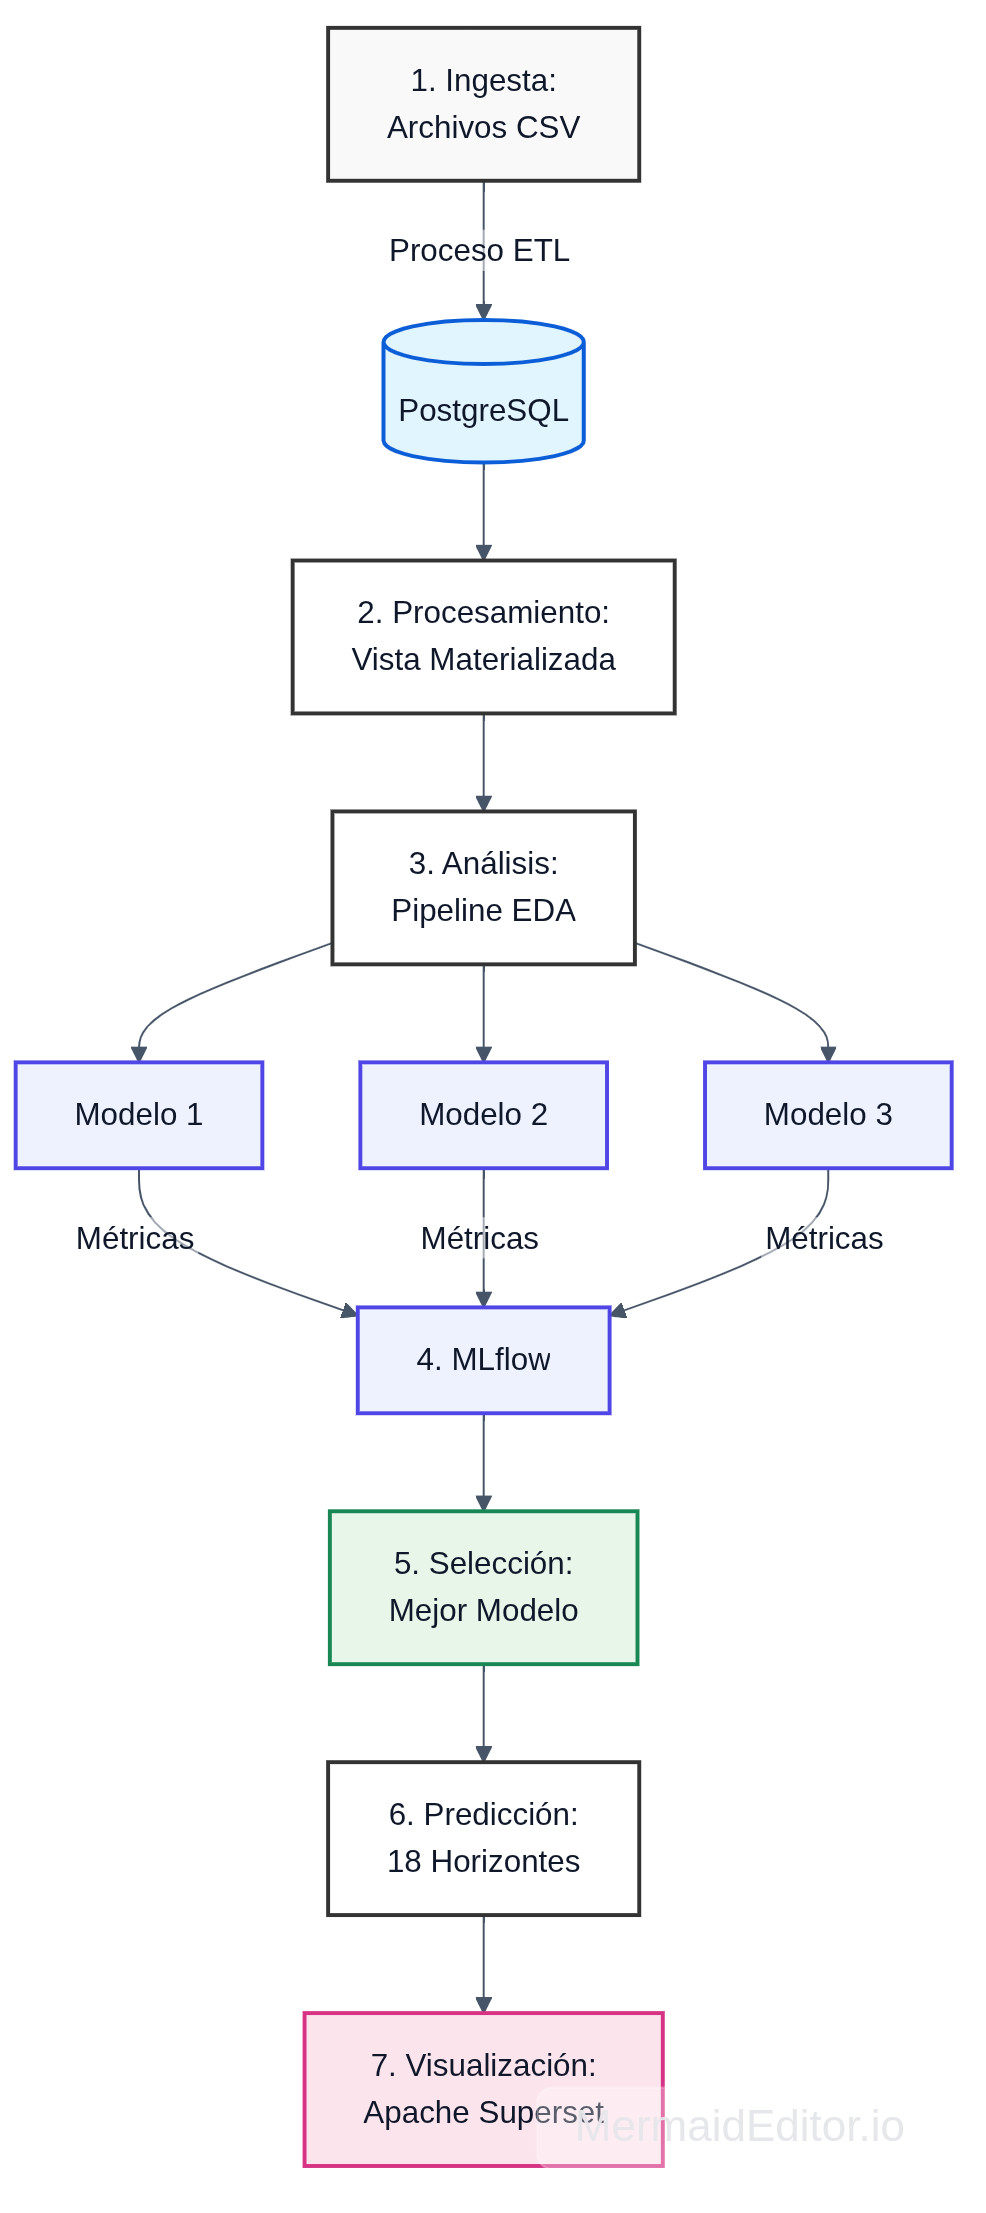
\includegraphics[width=0.45\linewidth]{images/mermaid-diagram.png}
    \caption{Diagrama de Arquitectura Propuesta}
    \label{fig:arquitectura}
\end{figure}

\begin{table}[h!]
    \centering
    \begin{tabular}{
        | >{\raggedright\arraybackslash}p{2.5cm}
        | >{\raggedright\arraybackslash}p{4.5cm}
        | >{\raggedright\arraybackslash}p{2.5cm}        
        | >{\raggedright\arraybackslash}p{4.5cm} |
    }
        \hline
            \textbf{Componente} & \textbf{Tecnología} & \textbf{Ubicación} & \textbf{Función} \\
        \hline
            Base de datos & PostgreSQL 15 \cite{postgresql2024documentation} & Local/Cloud & Datamart analítico \\
        \hline
            Orquestación & Apache Airflow 2.10 \cite{apache2024airflow} & Local/Cloud & Flujo de entrenamiento e inferencia \\
        \hline
            Tracking ML & MLflow \cite{mlflow2024documentation} & PC local & Registro de experimentos \\
        \hline
            Dashboards & Apache Superset \cite{apache2024superset} & Local/Cloud & Visualización BI \\
        \hline
            Entrenamiento & Python 3.12 + Jupyter & PC Local & Desarrollo de modelos \\
        \hline
    \end{tabular}
    \caption{Componentes del sistema y tecnologías utilizadas.}
    \label{tab:componentes}
\end{table}

La implementación incluye un flujo mensual de entrenamiento y un flujo diario de inferencia. Esta frecuencia corresponde a la configuración del prototipo; la tesis no presenta una evaluación de carga que demuestre que dichas periodicidades sean óptimas.

\section{Fuentes de datos y unidad de análisis}

El proceso ETL integra tres fuentes institucionales.

\begin{table}[h!]
    \centering
    \begin{tabular}{        
        | >{\raggedright\arraybackslash}p{6.5cm}
        | >{\raggedright\arraybackslash}p{3.5cm}        
        | >{\raggedright\arraybackslash}p{4.5cm} |   
    }
    \hline
        \textbf{Fuente} & \textbf{Magnitud} & \textbf{Contenido} \\
    \hline
        CABECERA\_PRESTAMOS & $\sim$500.000 filas & Información maestra de créditos, periodo 2015--2026 \\
    \hline
        AMORTIZACAL\_PRESTAMOS & $\sim$2.000.000 filas & Tabla de amortización mensual \\
    \hline
        RECUPERACION\_PRESTAMOS & $\sim$100.000 filas & Información de juicios y recuperaciones \\
    \hline
    \end{tabular}
    \caption{Fuentes de datos utilizadas en el proceso ETL.}
    \label{tab:fuentes_datos}
\end{table}

La Tabla 4.2b documenta la trazabilidad de los datos desde las fuentes hasta las muestras de entrenamiento, extraída del análisis del código fuente.

\begin{table}[h!]
\centering
\small
\begin{tabular}{|l|l|p{5cm}|}
\hline
\textbf{Etapa} & \textbf{Conteo} & \textbf{Descripción} \\
\hline
Filas CABECERA\_PRESTAMOS & $\sim$500.000 & Registros maestros de créditos \\
\hline
Filas AMORTIZACAL\_PRESTAMOS & $\sim$2.000.000 & Cuotas de amortización \\
\hline
Filas RECUPERACION\_PRESTAMOS & $\sim$100.000 & Juicios y recuperaciones \\
\hline
Filas tras integración (JOIN) & -- & Inner join creditos-amortizacion, left join juicios \\
\hline
Bloques-mes en MV & 20.025 & GROUP BY mes, riesgo, sector, sucursal \\
\hline
Bloques con historial $\geq 24$ meses & -- & Requerido: ventana(6) + horizontes(18) \\
\hline
Secuencias generadas & -- & \texttt{X\_cnn.shape[0]} (variable por ejecución) \\
\hline
Conjunto entrenamiento (49\%) & -- & 70\% inicial $\times$ 70\% interno \\
\hline
Conjunto validación (21\%) & -- & 30\% del train para early stopping \\
\hline
Conjunto prueba (30\%) & -- & Reservado para evaluación final \\
\hline
\end{tabular}
\caption{Trazabilidad de datos: transformación desde fuentes hasta conjuntos de entrenamiento. Los conteos exactos deben verificarse en el repositorio.}
\label{tab:trazabilidad}
\end{table}

\textbf{Nota}: La restricción clave es que solo los bloques con al menos 24 meses de historial (6 meses de ventana + 18 horizontes) generan secuencias válidas. Esto reduce significativamente el número de muestras disponibles desde los 20.025 bloques-mes iniciales.

\section{Procesamiento y preparación de datos}

El procesamiento se implementa en una vista materializada y en tareas del DAG. Las etapas documentadas son: integración de las tres fuentes, validación de claves, prevención de duplicados mediante upsert, agregación mensual y cálculo de características. El proyecto no aporta un registro completo de filas eliminadas, valores faltantes, criterios de tratamiento de atípicos ni conteos posteriores a cada filtro. Estas decisiones deben versionarse junto con el código para garantizar reproducibilidad.

Las redes neuronales requieren una representación secuencial. Para cada bloque se utiliza una ventana de seis meses con veintiuna características por mes, lo que corresponde a una matriz de $6 \times 21$ y a 126 valores antes de cualquier transformación adicional. La referencia original a 128 valores se corrige porque no se documentan dos variables adicionales.

\section{Ingeniería de características y variable objetivo}

El proyecto calcula veintiuna características numéricas derivadas de las tres fuentes. La Tabla 4.3 presenta el diccionario completo extraído del código fuente.

\begin{table}[h!]
\centering
\small
\begin{tabular}{|l|l|p{5cm}|}
\hline
\textbf{Variable} & \textbf{Grupo} & \textbf{Interpretación} \\
\hline
num\_creditos & Volumen & Número de créditos agregados en el bloque-mes \\
\hline
monto\_total & Volumen & Suma del monto crediticio \\
\hline
monto\_promedio & Volumen & Monto promedio de los créditos \\
\hline
plazo\_promedio & Condición & Plazo promedio de las operaciones (cuotas) \\
\hline
tasa\_interes\_promedio & Condición & Tasa de interés promedio \\
\hline
saldo\_promedio & Riesgo & Saldo capital promedio \\
\hline
total\_costo\_judicial & Riesgo & Suma de costos judiciales del bloque \\
\hline
total\_gestion\_cobro & Riesgo & Suma de gestiones de cobro \\
\hline
total\_notificaciones & Riesgo & Suma de notificaciones \\
\hline
tot\_dias\_mora\_promedio & Riesgo & Promedio de días en mora \\
\hline
tot\_num\_moras\_promedio & Riesgo & Promedio de número de moras \\
\hline
mora\_promedio & Riesgo & Monto promedio de mora \\
\hline
creditos\_judiciales & Riesgo & Créditos con indicador judicial = `S' \\
\hline
creditos\_cerrados & Riesgo & Créditos con estado `C' o `L' \\
\hline
tasa\_judicial & Riesgo & creditos\_judiciales / num\_creditos $\times$ 100 \\
\hline
tasa\_cierre & Riesgo & creditos\_cerrados / num\_creditos $\times$ 100 \\
\hline
tasa\_mora\_90 & Riesgo & Créditos con $>$90 días mora / num\_creditos $\times$ 100 \\
\hline
creditos\_por\_cliente & Derivada & num\_creditos / num\_clientes\_unicos \\
\hline
coef\_variacion\_montos & Derivada & desviación\_montos / monto\_promedio $\times$ 100 \\
\hline
tasa\_crecimiento\_creditos & Derivada & Variación \%, $\Delta$ num\_creditos / num\_creditos\_previo \\
\hline
tasa\_crecimiento\_monto & Derivada & Variación \%, $\Delta$ monto\_total / monto\_total\_previo \\
\hline
\end{tabular}
\caption{Diccionario completo de las 21 características extraído del código fuente (\texttt{queries.py} y pipelines de modelos).}
\label{tab:caracteristicas}
\end{table}

La variable binaria \texttt{crisis\_flag} se construye mediante ocho condiciones heurísticas con pesos acumulativos. Si la suma de pesos supera el umbral de 5, el bloque se etiqueta como crisis (1); de lo contrario, como no crisis (0). Las ocho condiciones son:

\begin{enumerate}
    \item \textbf{Condición 1} (peso 3): tasa\_judicial $> 5\%$
    \item \textbf{Condición 2} (peso 1): tasa\_judicial $> 2\%$
    \item \textbf{Condición 3} (peso 2): costo\_judicial $> 0$ Y (costo\_judicial / num\_creditos) $> $ monto\_promedio $\times$ 10\%
    \item \textbf{Condición 4} (peso 1): gestión\_cobro $> 0$ Y (gestión\_cobro / num\_creditos) $> $ monto\_promedio $\times$ 5\%
    \item \textbf{Condición 5} (peso 2 o 1): tasa\_cierre $> 30\%$ (peso 2) o $> 20\%$ (peso 1)
    \item \textbf{Condición 6} (peso 1): plazo\_promedio $> 36$ meses
    \item \textbf{Condición 7} (peso 1): plazo\_promedio $> 60$ meses
    \item \textbf{Condición 8} (peso 1): tasa\_interes\_promedio $> 15\%$
\end{enumerate}

Umbral de decisión: $\sum \text{pesos} \geq 5 \Rightarrow \texttt{crisis\_flag} = 1$. La etiqueta fue validada por juicio experto según el documento original, aunque el procedimiento de validación no está documentado.

\begin{figure}[H]
    \centering
    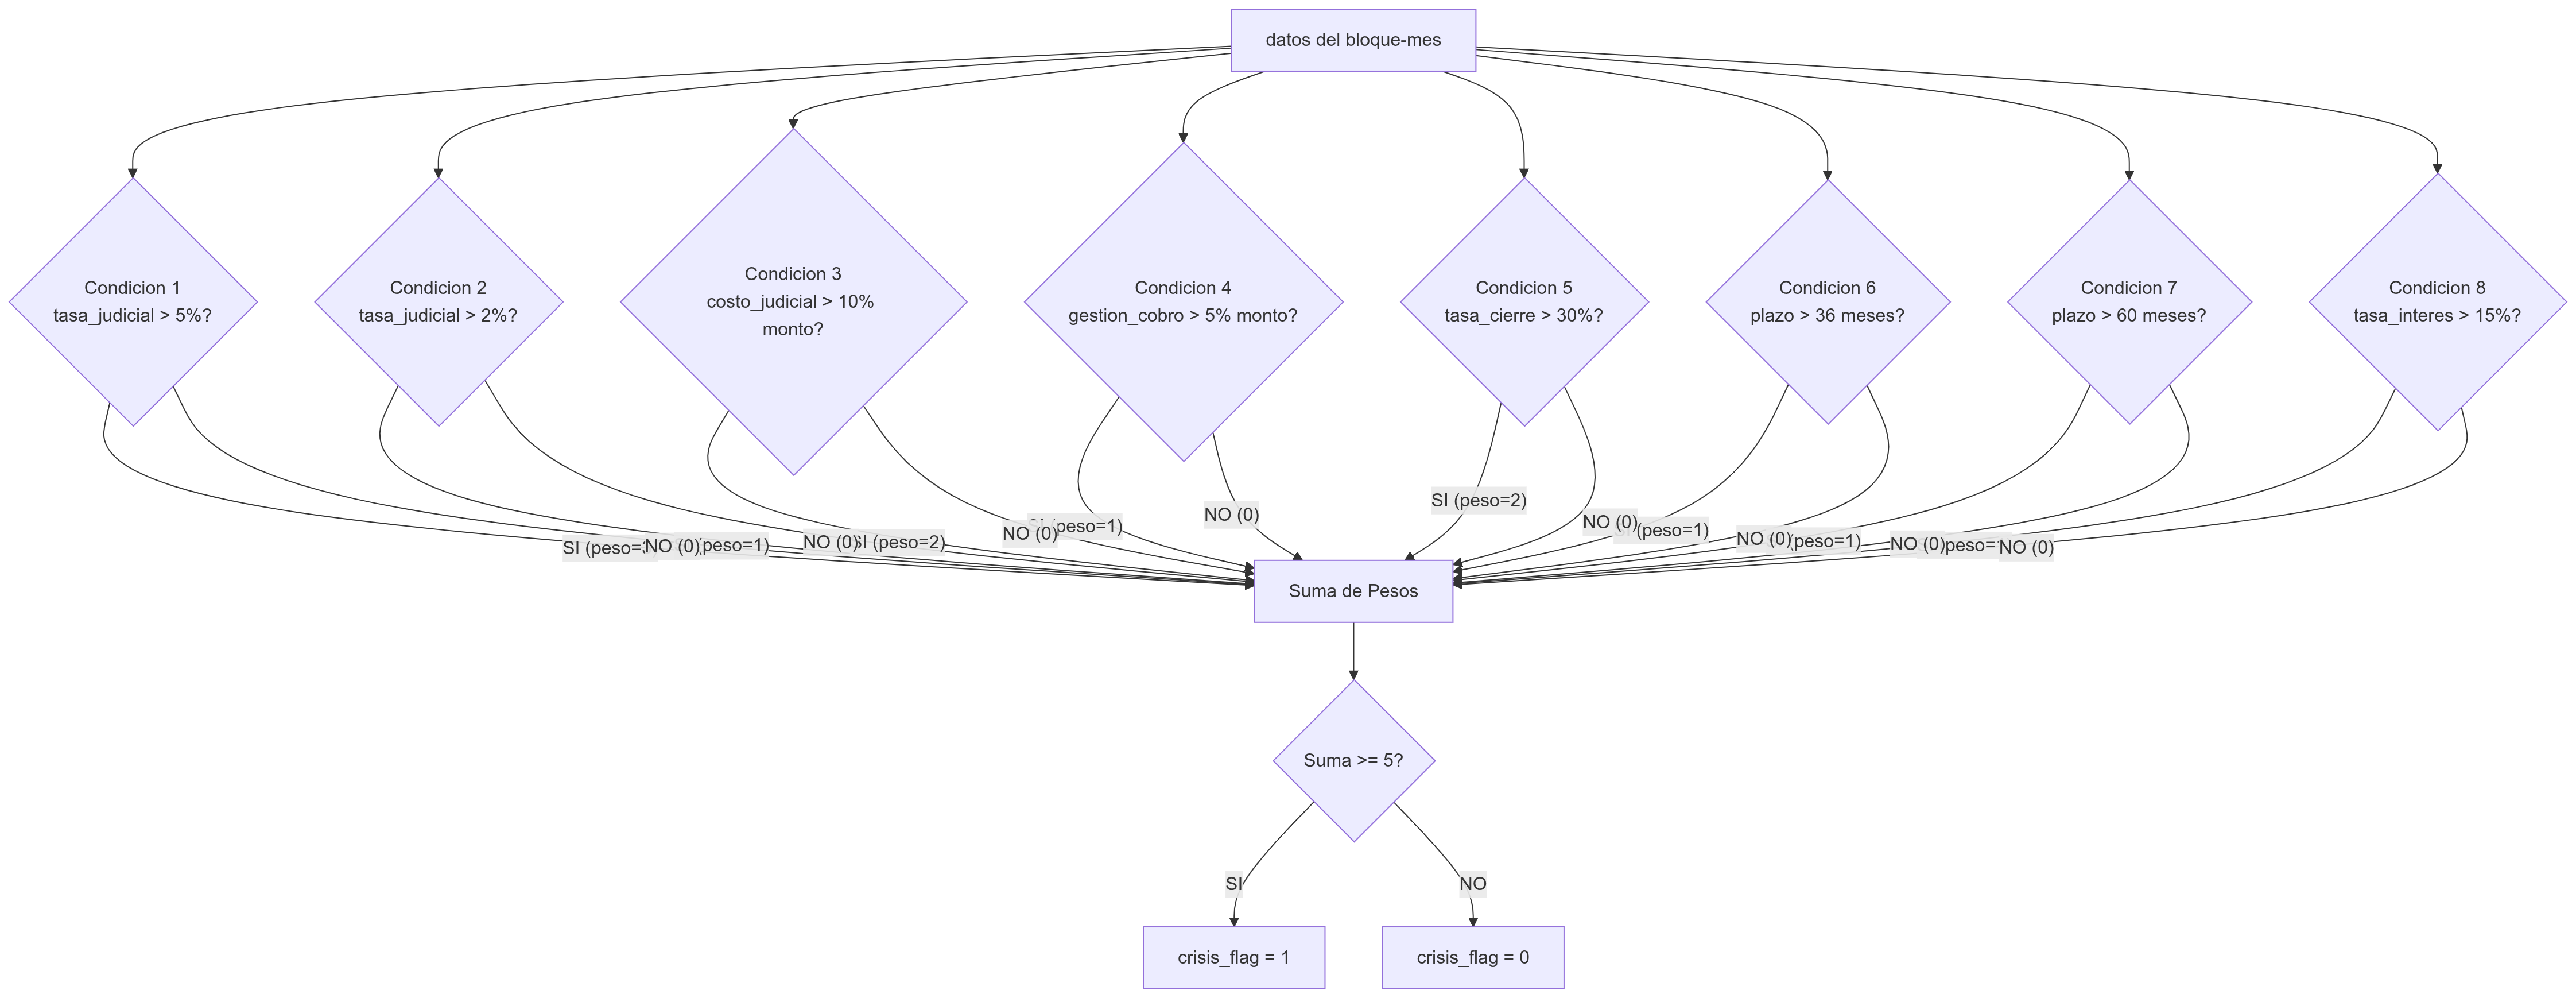
\includegraphics[width=0.8\linewidth]{images/MM-07 Definicion de crisis_flag.png}
    \caption{Diagrama de flujo de la definición de \texttt{crisis\_flag}. Cada condición evalúa un umbral y asigna un peso; si la suma total supera 5, el bloque se etiqueta como crisis.}
    \label{fig:crisis_flag}
\end{figure}

\textbf{Advertencia de fuga de información}: Las condiciones 1, 2 y 3 utilizan variables judiciales (\texttt{creditos\_judiciales}, \texttt{tasa\_judicial}, \texttt{total\_costo\_judicial}) que también aparecen como características de entrada. Esto crea una dependencia directa entre la etiqueta y algunas variables predictoras, lo que constituye un riesgo de target leakage. Las variables judiciales muestran un poder predictivo elevado (AUC individual $> 0,9$) parcialmente porque contribuyen a la definición de la etiqueta. Se recomienda una ablación excluyendo estas variables para estimar su impacto real.

\subsection{Generación de horizontes}

La salida considera dieciocho horizontes mensuales. Para una ventana que termina en $t$, la etiqueta del horizonte $h$ corresponde al estado futuro en $t + h$. CNN y MLP generan un vector de dieciocho probabilidades, mientras que LightGBM entrena un clasificador independiente por horizonte.

\begin{figure}[H]
    \centering
    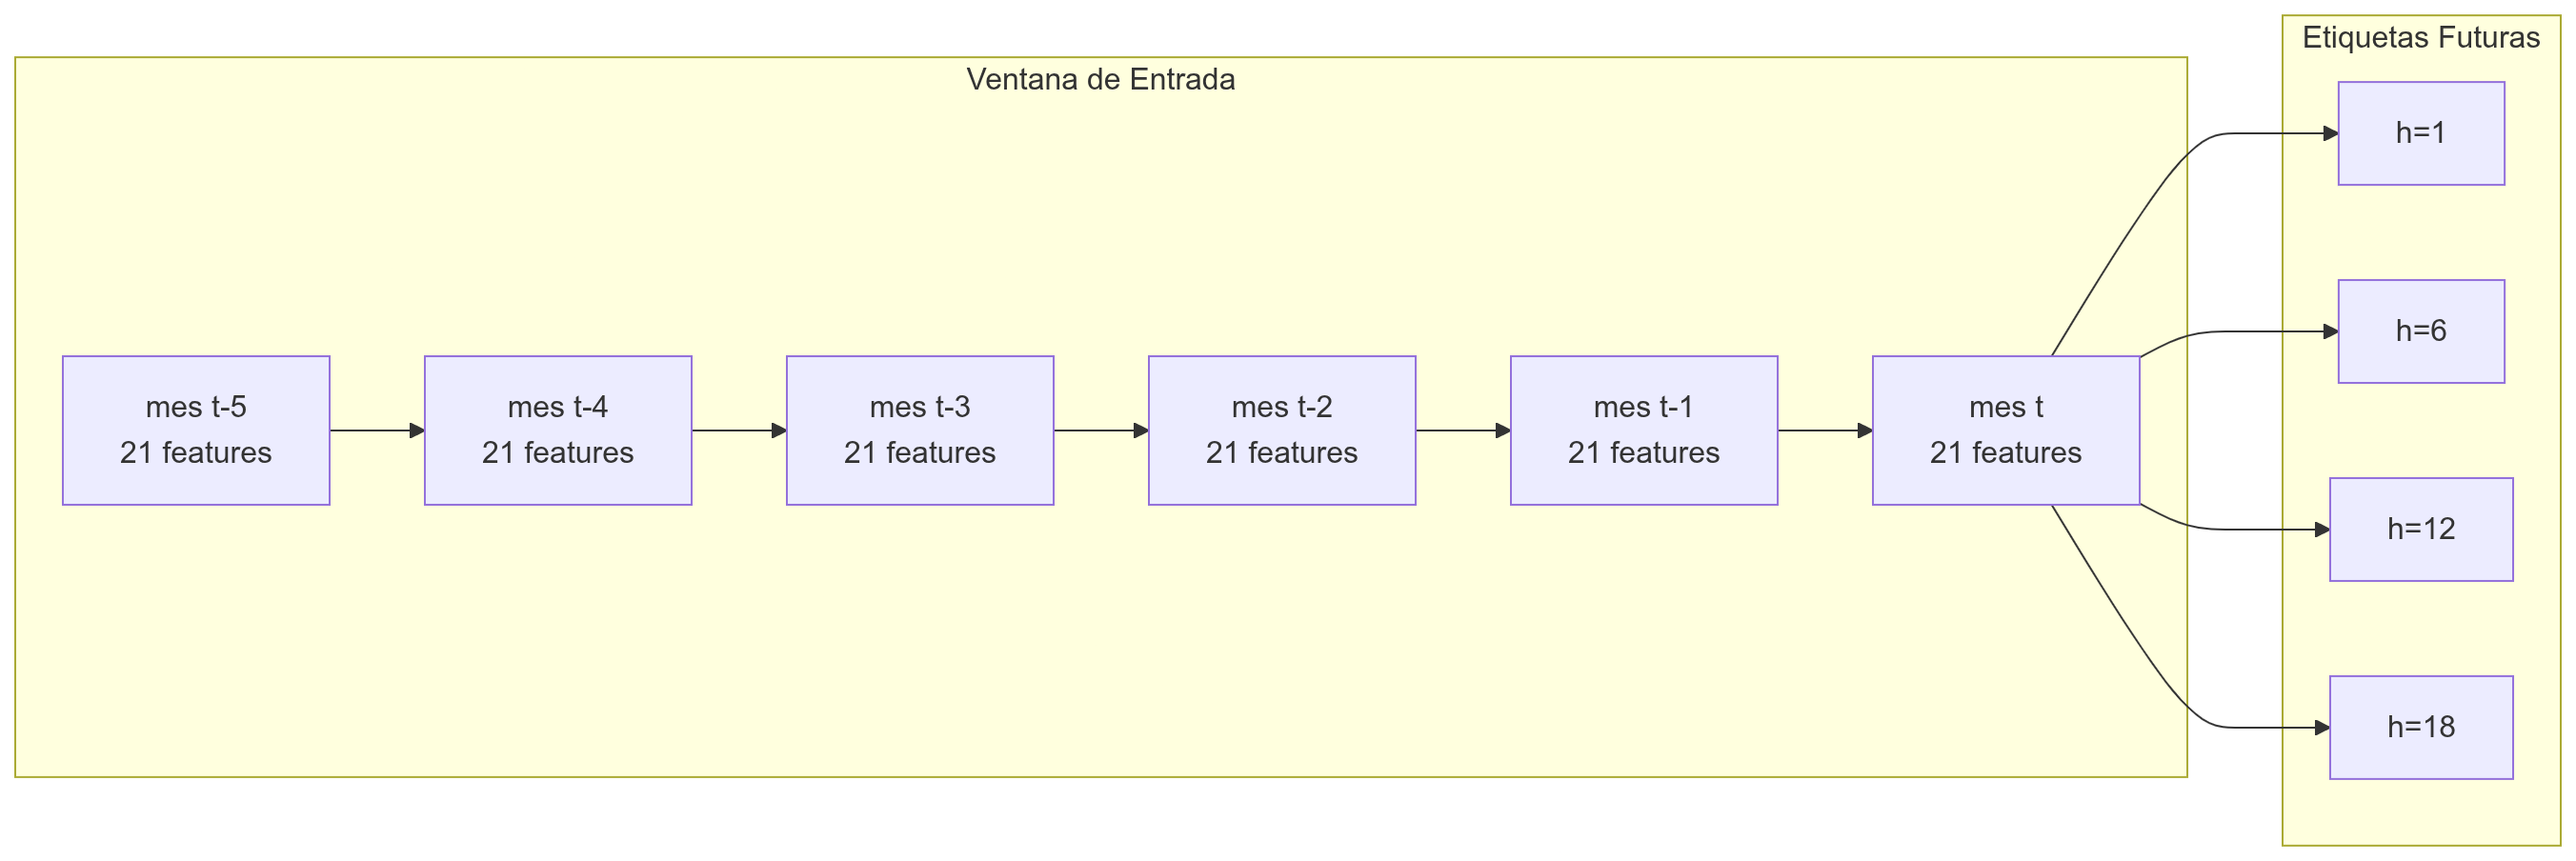
\includegraphics[width=0.8\linewidth]{images/MM-01 Ventana Temporal de Entrada (6 meses × 21 features).png}
    \caption{Representación conceptual de la ventana de entrada y las etiquetas multi-horizonte. Cada bloque-mes genera una secuencia de 6 meses con 21 características, y 18 etiquetas futuras correspondientes a los horizontes de predicción.}
    \label{fig:horizontes}
\end{figure}

\section{Algoritmos seleccionados}

Se comparan tres familias para representar enfoques distintos sobre los mismos datos tabulares y temporales.

\subsection{CNN multi-horizonte}

La CNN se implementa como una red unidimensional (\texttt{Conv1D}) con la siguiente arquitectura completa extraída del código fuente:

\begin{itemize}
    \item \texttt{Input}: ventana de $6 \times 21$ (6 meses, 21 características)
    \item \texttt{Conv1D(64, kernel\_size=3, activation=`relu', padding=`same')}
    \item \texttt{BatchNormalization}
    \item \texttt{Dropout(0.3)}
    \item \texttt{Conv1D(128, kernel\_size=3, activation=`relu', padding=`same')}
    \item \texttt{BatchNormalization}
    \item \texttt{MaxPooling1D(pool\_size=2)}
    \item \texttt{Dropout(0.3)}
    \item \texttt{Flatten}
    \item \texttt{Dense(128, activation=`relu')}
    \item \texttt{BatchNormalization}
    \item \texttt{Dropout(0.4)}
    \item \texttt{Dense(64, activation=`relu')}
    \item \texttt{Dropout(0.3)}
    \item 18 salidas \texttt{Dense(1, activation=`sigmoid')}, una por horizonte
\end{itemize}

Configuración de entrenamiento:
\begin{itemize}
    \item Pérdida: \texttt{binary\_crossentropy}
    \item Optimizador: Adam (lr por defecto = 0,001)
    \item Épocas máximas: 100
    \item Batch size: 32
    \item Early stopping: paciencia = 10, monitorea \texttt{val\_loss}, restaura mejores pesos
    \item Sample weights: SÍ calcula pesos por clase (\texttt{total / (2 $\times$ n\_clase)})
    \item Escalado: MinMaxScaler (fit solo en train)
    \item Tratamiento de atípicos: clipping a quantiles 0,01--0,99
\end{itemize}

\subsection{MLP multi-horizonte}

El MLP se implementa como un perceptrón multicapa con aplanamiento de la secuencia temporal. La arquitectura completa es:

\begin{itemize}
    \item \texttt{Input}: ventana de $6 \times 21$
    \item \texttt{Flatten} (aplana a vector de 126 elementos)
    \item \texttt{Dense(128, activation=`relu')}
    \item \texttt{Dropout(0.3)}
    \item \texttt{Dense(64, activation=`relu')}
    \item \texttt{Dropout(0.2)}
    \item 18 salidas \texttt{Dense(1, activation=`sigmoid')}, una por horizonte
\end{itemize}

Configuración de entrenamiento:
\begin{itemize}
    \item Pérdida: \texttt{binary\_crossentropy}
    \item Optimizador: Adam (lr = 0,001)
    \item Épocas máximas: 100
    \item Batch size: 32
    \item Early stopping: paciencia = 10, monitorea \texttt{val\_loss}, restaura mejores pesos
    \item Sample weights: NO utiliza ponderación por clase (a diferencia de CNN)
    \item Escalado: MinMaxScaler (fit solo en train)
    \item Tratamiento de atípicos: clipping a quantiles 0,01--0,99
\end{itemize}

\textbf{Diferencia crítica con CNN}: El MLP no implementa \texttt{sample\_weights}, lo que significa que el desbalance de clases (85\% no crisis vs 15\% crisis) no se compensa durante el entrenamiento. Esta omisión puede explicar parcialmente por qué el MLP predice todas las observaciones como ``no crisis''.

\subsection{LightGBM multi-horizonte}

LightGBM se implementa mediante dieciocho clasificadores independientes, uno por horizonte, siguiendo los principios de gradient boosting \cite{friedman2001greedy, ke2017lightgbm}. La configuración completa extraída del código es:

\begin{itemize}
    \item \texttt{objective}: binary
    \item \texttt{metric}: binary\_logloss
    \item \texttt{boosting\_type}: gbdt
    \item \texttt{num\_leaves}: 31
    \item \texttt{learning\_rate}: 0,05
    \item \texttt{feature\_fraction}: 0,8
    \item \texttt{bagging\_fraction}: 0,8
    \item \texttt{bagging\_freq}: 5
    \item \texttt{seed}: 42 (semilla fija para reproducibilidad)
    \item \texttt{n\_jobs}: -1 (usa todos los núcleos)
    \item Early stopping: 50 rondas sin mejora
    \item Número máximo de boost rounds: 1000
    \item Escalado: MinMaxScaler (fit solo en train)
\end{itemize}

A diferencia de las redes neuronales, LightGBM no requiere representación secuencial; cada horizonte se entrena como un problema de clasificación binaria independiente con las mismas 21 características.

\begin{table}
\centering
\small
\begin{tabular}{|l|l|l|l|}
\hline
\textbf{Elemento} & \textbf{LightGBM} & \textbf{CNN} & \textbf{MLP} \\
\hline
Salida & 18 modelos binarios independientes & 18 salidas sigmoidales & 18 salidas sigmoidales \\
\hline
Arquitectura & Árboles potenciados (GBDT) & Conv1D(64,$k$=3), BN, Do(0,3), Conv1D(128,$k$=3), BN, MaxPool(2), Do(0,3), Flat, Den(128), BN, Do(0,4), Den(64), Do(0,3) & Flat, Den(128), Do(0,3), Den(64), Do(0,2) \\
\hline
Optimizador & GBDT, lr=0,05 & Adam (lr=0,001) & Adam (lr=0,001) \\
\hline
Loss & binary\_logloss & binary\_crossentropy & binary\_crossentropy \\
\hline
Batch size & N/A (usa bagging) & 32 & 32 \\
\hline
Sample weights & scale\_pos\_weight=5,67 & SÍ (total/2$\times$n\_clase) & NO \\
\hline
Early stopping & 50 rondas & Paciencia 10 (\texttt{val\_loss}) & Paciencia 10 (\texttt{val\_loss}) \\
\hline
Semilla & 42 (fija) & No fijada & No fijada \\
\hline
Escalado & MinMaxScaler & MinMaxScaler & MinMaxScaler \\
\hline
Clipping & No & SÍ (q01--q99) & SÍ (q01--q99) \\
\hline
\end{tabular}
\caption{Configuración completa documentada de los modelos evaluados, extraída del código fuente.}
\label{tab:config_modelos}
\end{table}

\begin{figure}[H]
    \centering
    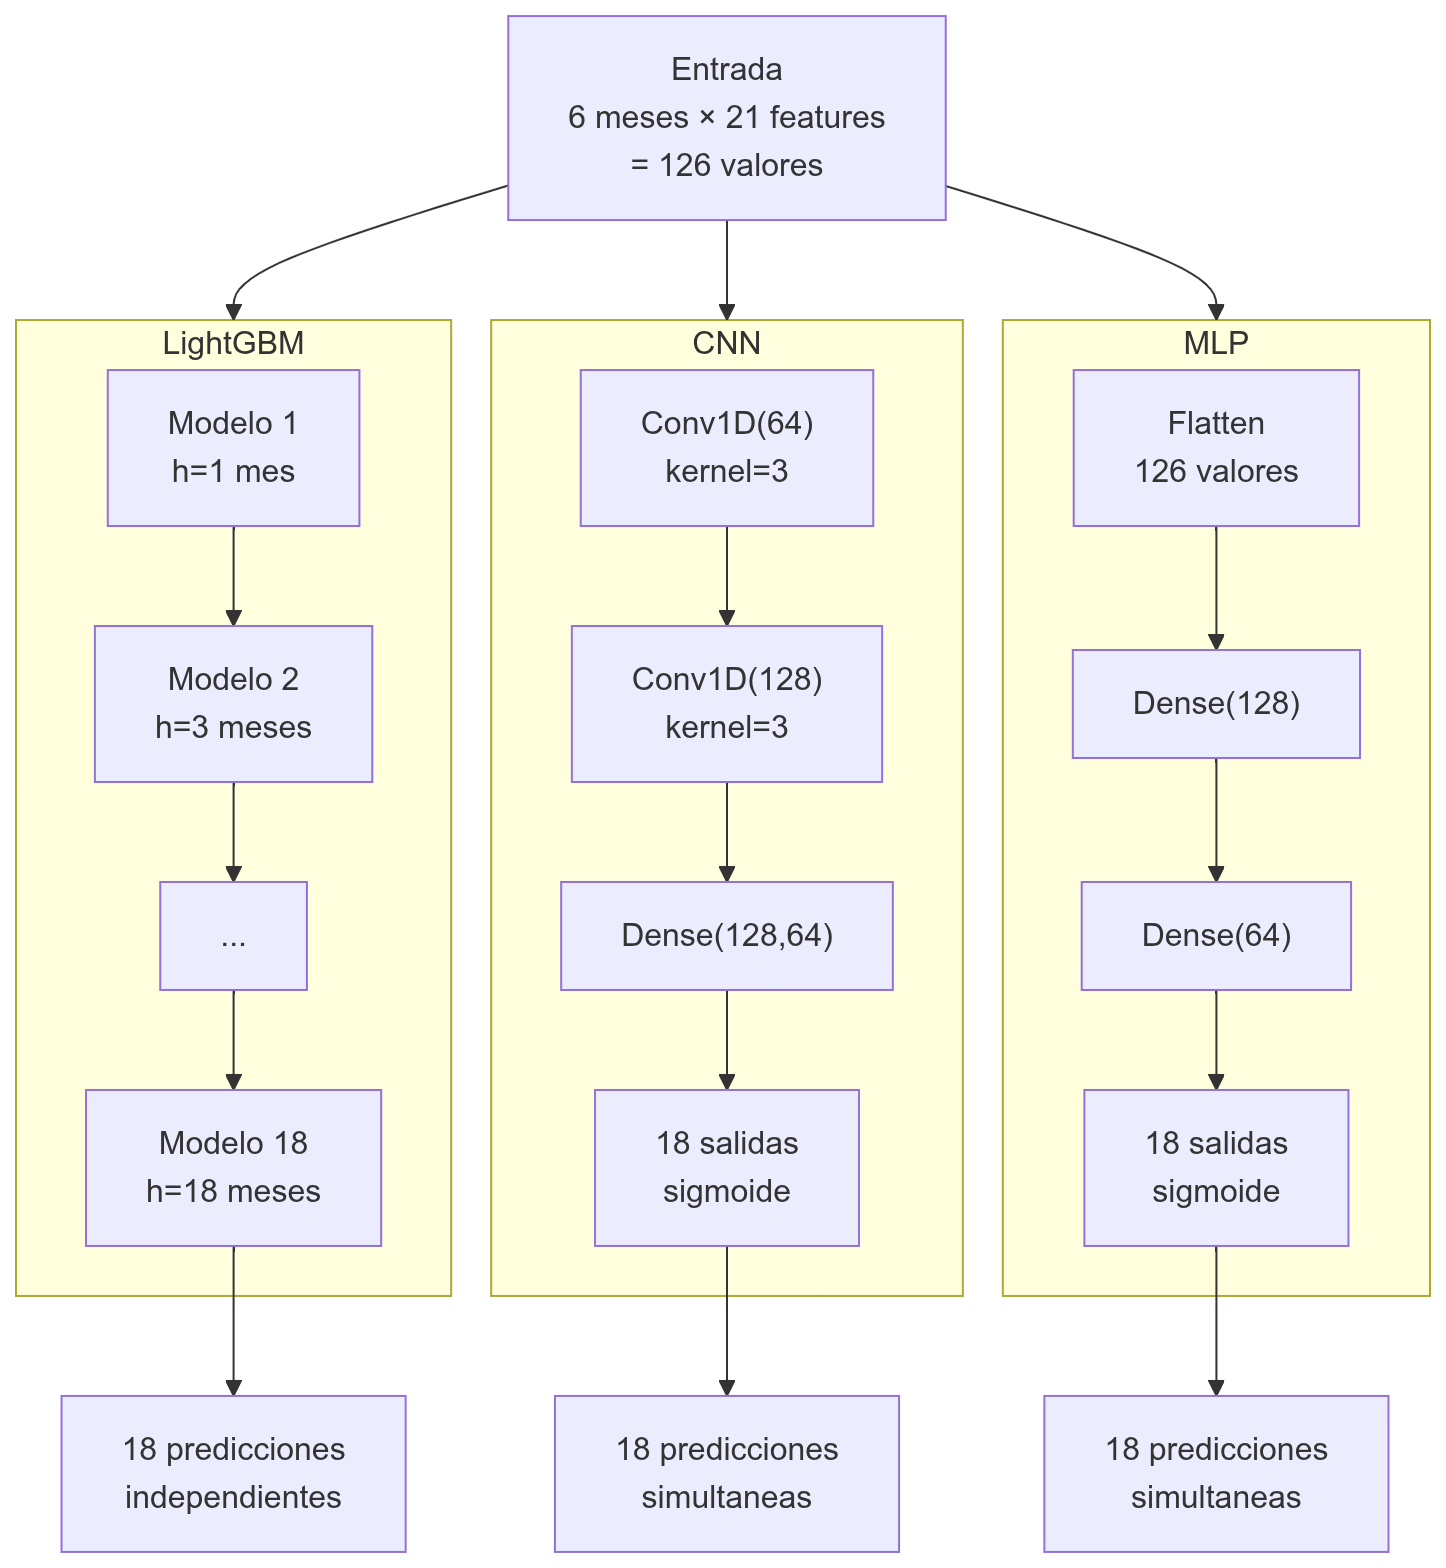
\includegraphics[width=0.8\linewidth]{images/MM-03 Comparacion de Arquitecturas de Modelos.png}
    \caption{Comparación de arquitecturas: LightGBM entrena 18 modelos independientes (uno por horizonte), mientras que CNN y MLP son redes únicas con 18 salidas sigmoidales. Todos comparten la misma entrada de $6 \times 21$ valores.}
    \label{fig:arquitecturas}
\end{figure}

\section{Hiperparámetros y estrategia de ajuste}

Los hiperparámetros de LightGBM se seleccionaron mediante búsqueda manual. No se documentan el espacio explorado, el número de configuraciones ni la regla utilizada para detener la búsqueda. Para CNN y MLP se reportan las arquitecturas principales, pero no un procedimiento equivalente de ajuste. Por ello, la comparación refleja las implementaciones disponibles y no una búsqueda equilibrada de la mejor configuración de cada familia.

El valor \texttt{scale\_pos\_weight=5,67} es consistente con una razón aproximada entre clases negativa y positiva, pero el cálculo exacto debe realizarse únicamente con el conjunto de entrenamiento de cada horizonte. El proyecto no presenta los conteos por horizonte necesarios para verificarlo.

\section{Protocolo de entrenamiento, validación y prueba}

La división de datos se implementa en tres etapas temporales, verificada en el código fuente:

\begin{enumerate}
    \item \textbf{División temporal inicial} (70\% / 30\%): Los datos se ordenan cronológicamente y se dividen en entrenamiento (70\% más antiguo) y prueba (30\% más reciente).
    \item \textbf{Extracción de validación} (del 70\% de train): Del conjunto de entrenamiento se extrae un 30\% para validación, resultando en:
\end{enumerate}

\begin{table}[h!]
\centering
\begin{tabular}{|l|l|l|}
\hline
\textbf{Conjunto} & \textbf{Proporción} & \textbf{Uso} \\
\hline
Entrenamiento & 49\% del total & Ajuste de pesos del modelo \\
\hline
Validación & 21\% del total & Early stopping, monitoreo de \texttt{val\_loss} \\
\hline
Prueba & 30\% del total & Evaluación final (una sola vez) \\
\hline
\end{tabular}
\caption{Distribución real de los conjuntos de datos extraída del código.}
\label{tab:splits}
\end{table}

\begin{figure}[H]
    \centering
    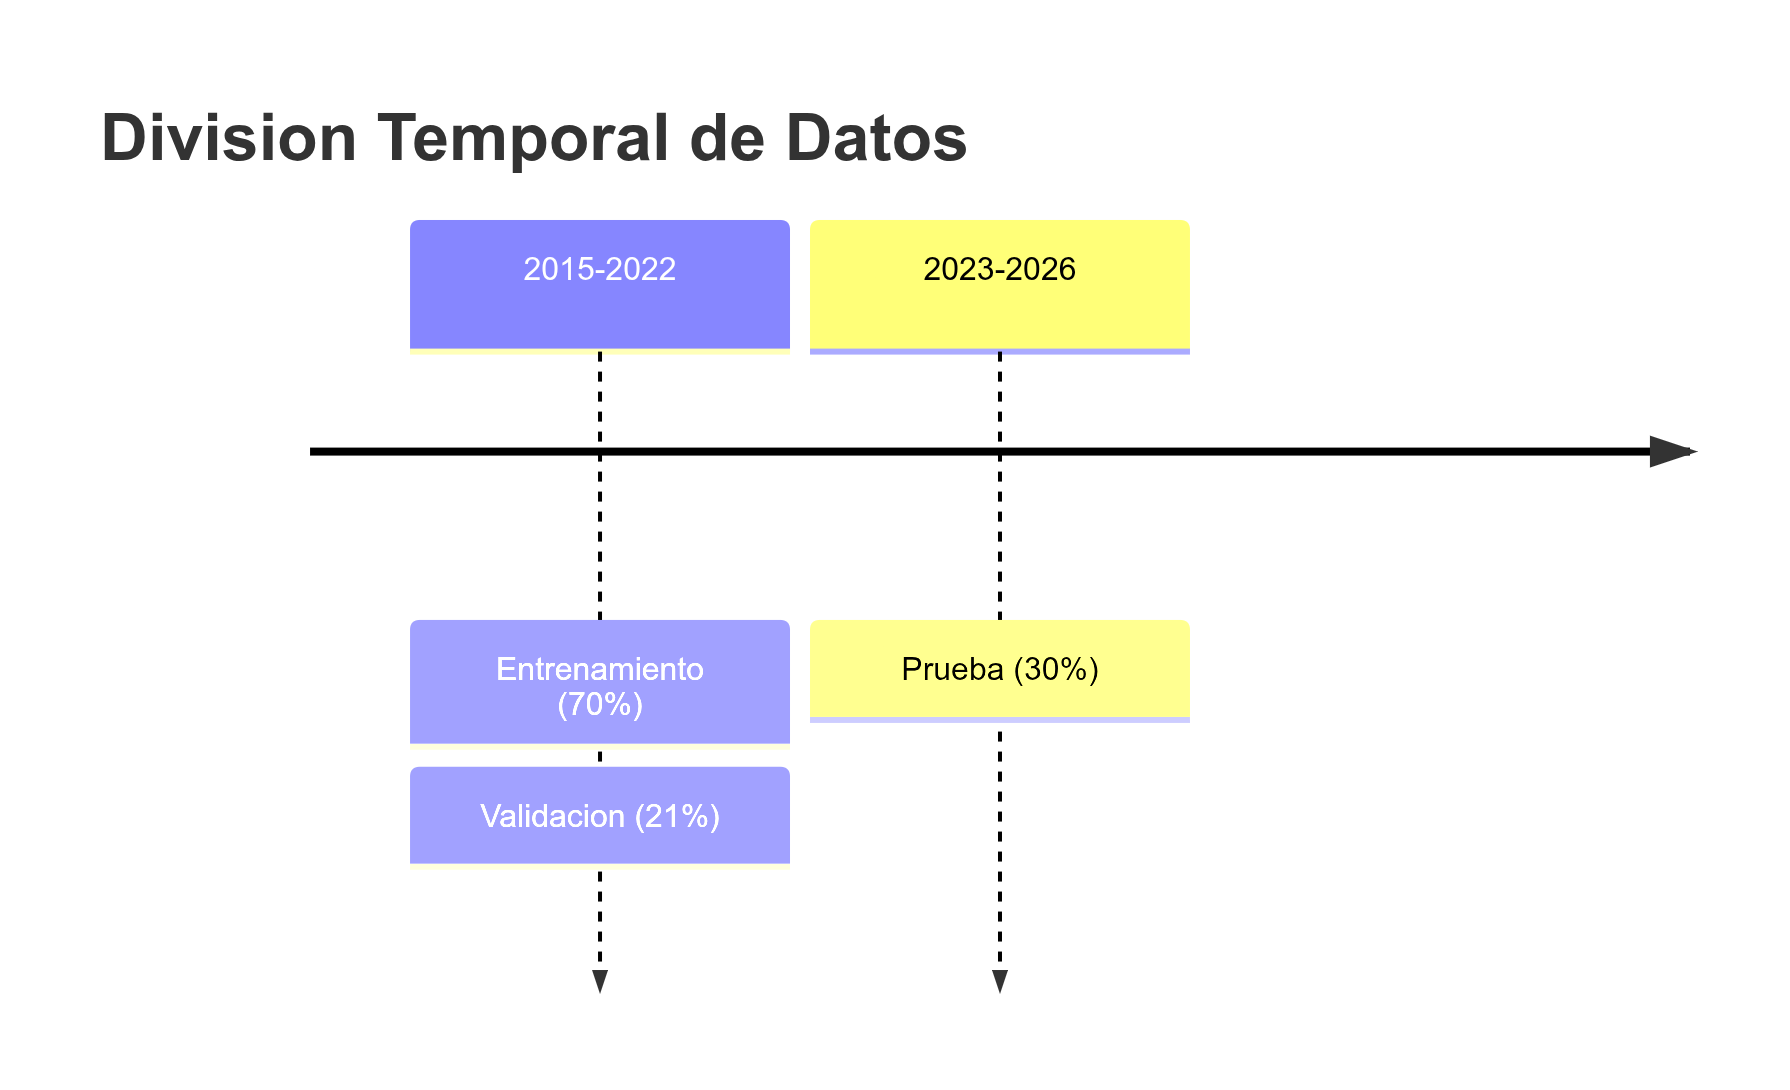
\includegraphics[width=0.8\linewidth]{images/MM-02 b Diagrama Linea Tiempo.png}
    \caption{Línea de tiempo de la división temporal de datos. El periodo 2015--2022 se utiliza para entrenamiento y validación, mientras que 2023--2026 se reserva para prueba.}
    \label{fig:timeline}
\end{figure}

El conjunto de validación se utiliza exclusivamente para early stopping (monitoreo de \texttt{val\_loss} con paciencia de 10 épocas) y checkpoint del mejor modelo. El conjunto de prueba se reserva para una única evaluación al final del entrenamiento.

\textbf{Limitaciones del protocolo}: (1) No se reportan los conteos exactos de muestras por conjuntos y por horizonte; (2) la semilla no está fijada para CNN y MLP, lo que dificulta la reproducibilidad; (3) no se realizan repeticiones con múltiples semillas para estimar variabilidad; (4) la búsqueda de hiperparámetros fue manual y no documentada.

\begin{figure}[H]
    \centering
    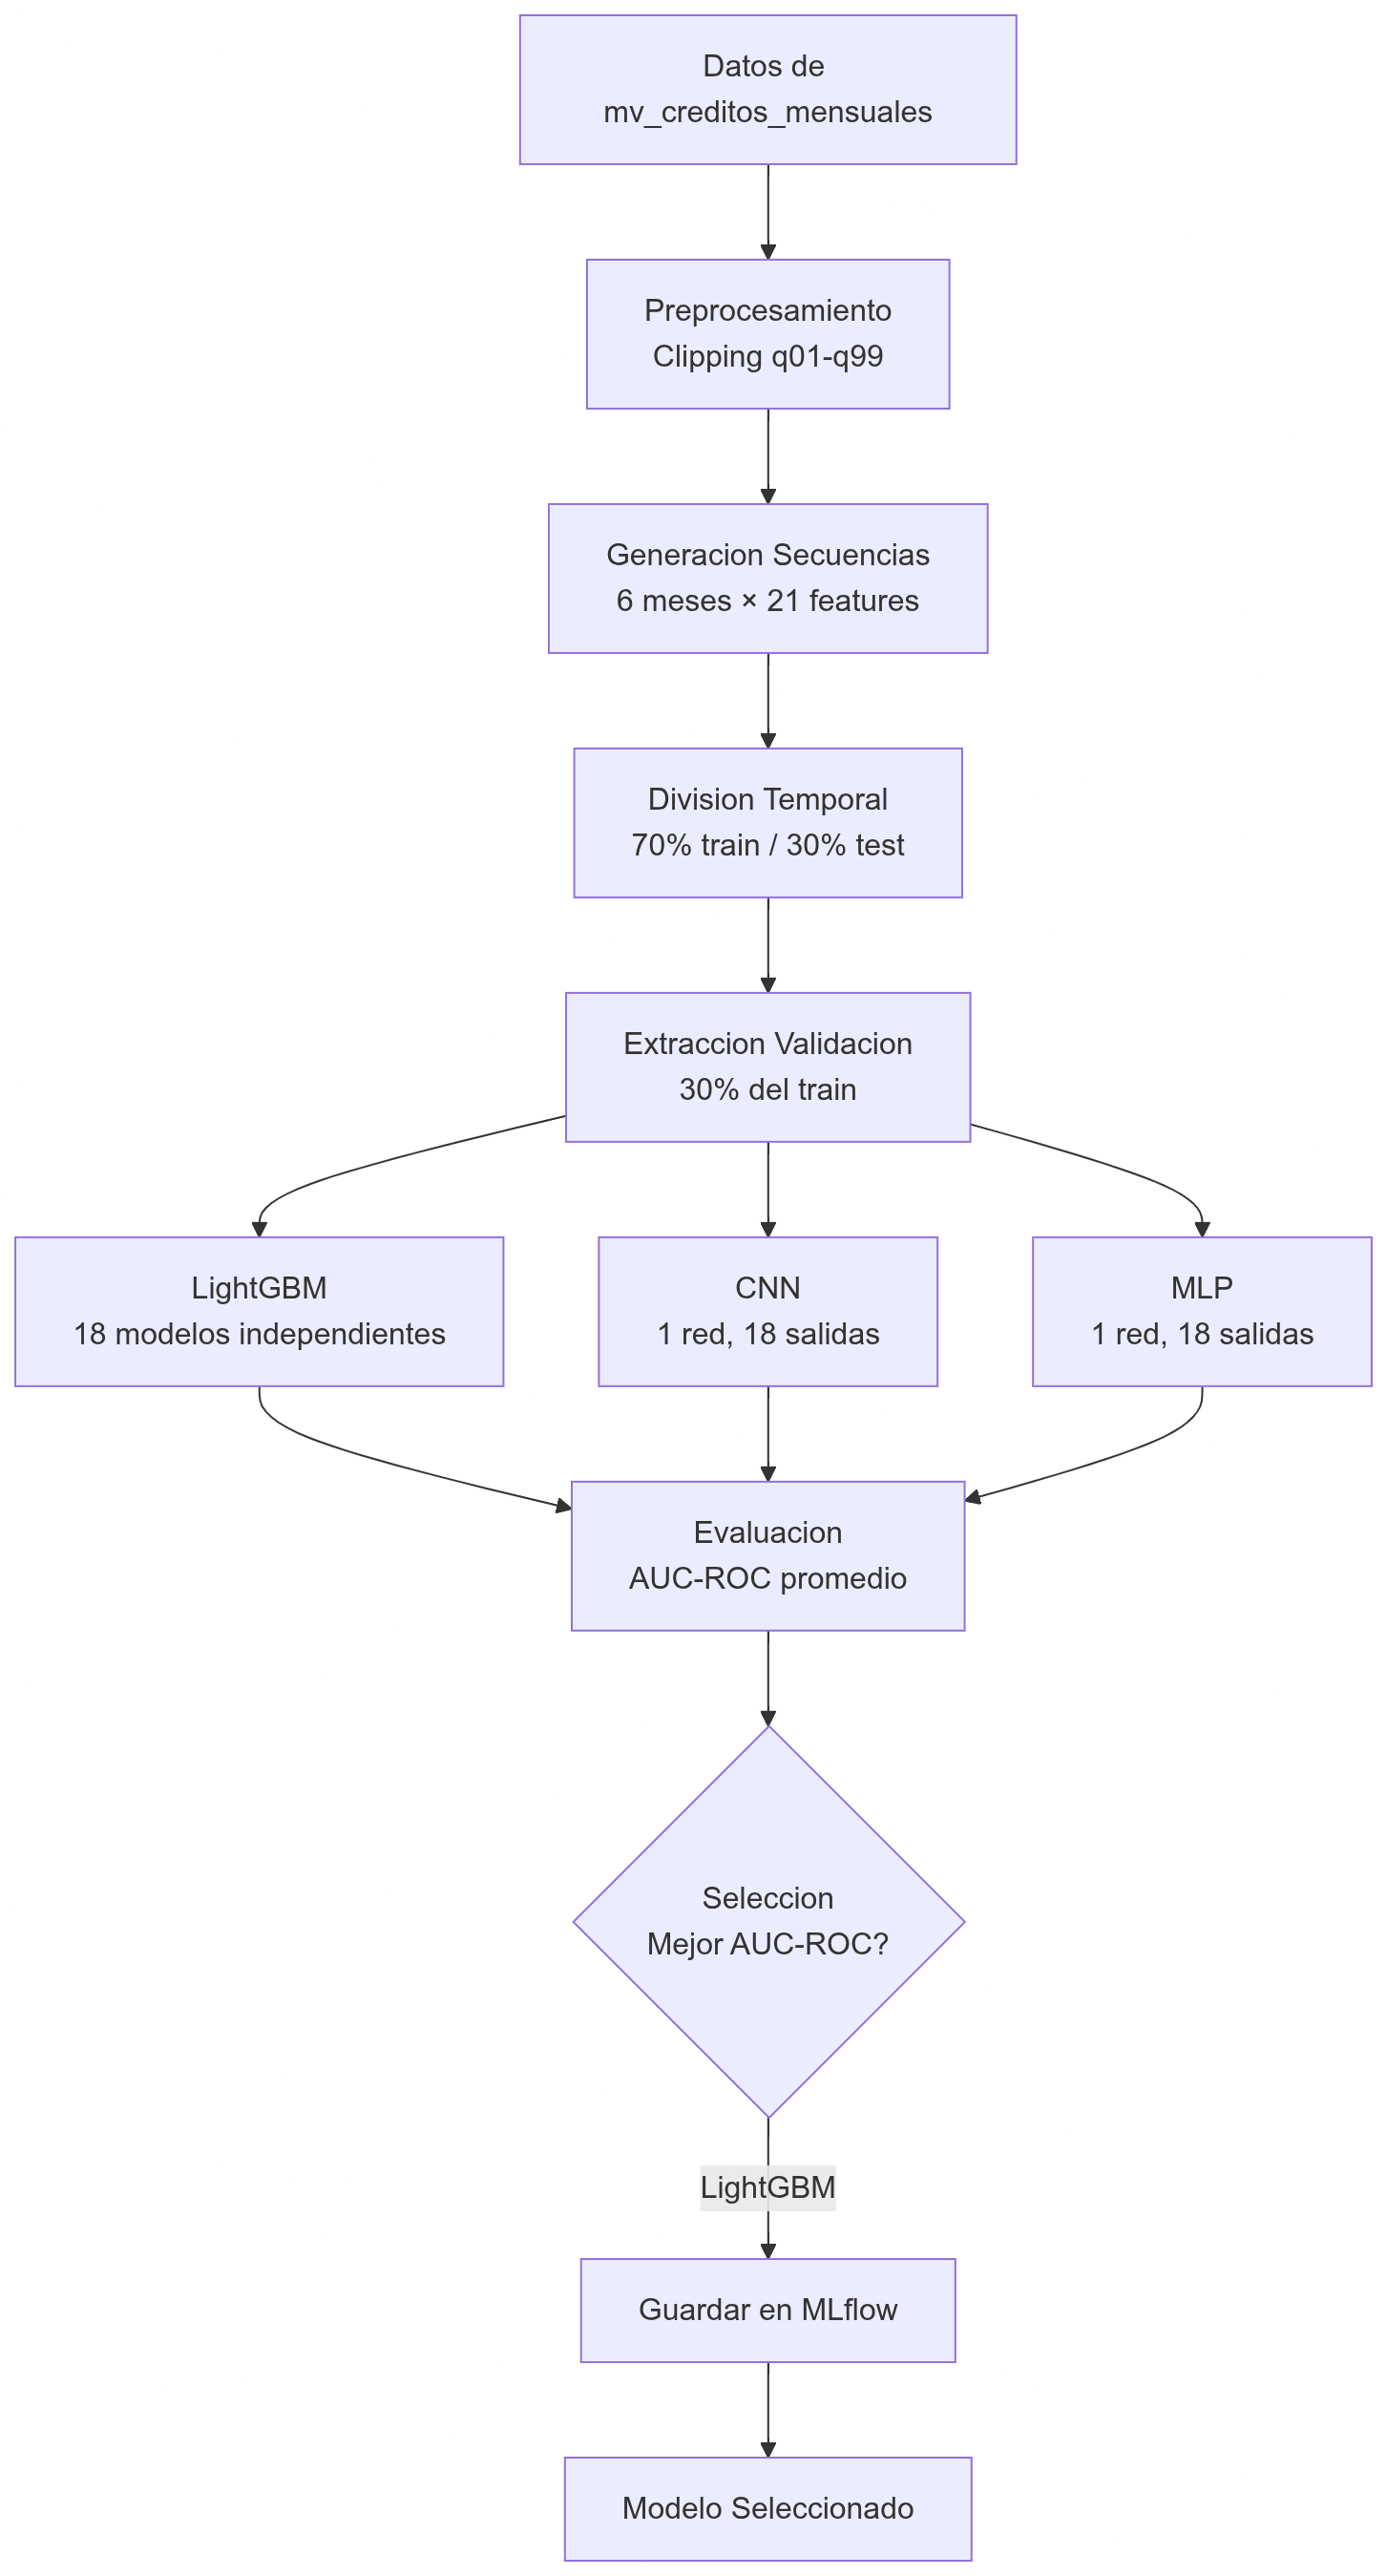
\includegraphics[width=0.8\linewidth]{images/MM-05 Flujo de Entrenamiento.png}
    \caption{Flujo de entrenamiento, registro y selección implementado en el prototipo. Los datos pasan por preprocesamiento, generación de secuencias y división temporal antes de entrenar los tres modelos.}
    \label{fig:entrenamiento}
\end{figure}

\section{Métricas y criterio de selección}

Los modelos se evalúan mediante accuracy, precision, recall, F1-score y AUC-ROC. El criterio principal implementado para seleccionar el modelo es el AUC-ROC promedio de los dieciocho horizontes registrado en MLflow. En la discusión se examina también el recall, debido a que un AUC moderado puede coexistir con una baja detección de crisis bajo el umbral utilizado.

No se reportan intervalos de confianza, pruebas estadísticas, PR-AUC ni calibración. En consecuencia, no se utiliza el término significativo en sentido estadístico y no se atribuyen diferencias observadas a una causa específica.

\section{Pipeline MLOps y registro de experimentos}

El DAG de entrenamiento se programa para el primer día de cada mes a las 03:00. Sus tareas cubren extracción, carga, preparación, entrenamiento, cálculo de métricas y registro de artefactos. La versión original ejecuta los modelos en paralelo; este diseño puede aumentar la utilización de recursos, pero no se dispone de mediciones de CPU, memoria o temperatura que permitan cuantificar el impacto.

MLflow almacena los resultados de las ejecuciones y permite recuperar el modelo seleccionado. La tesis no documenta un esquema de aprobación humana verificable, reglas de promoción, hash de datos, commit del código ni política de reversión. Por ello, el sistema se presenta como prototipo MLOps y no como una operación regulada en producción.

\section{Puesta en producción e inferencia}

El DAG de inferencia se ejecuta diariamente a las 06:00. Actualiza la vista materializada, carga el modelo registrado, genera probabilidades para los dieciocho horizontes y realiza upsert en \texttt{fact\_predicciones\_mensual}.

\begin{figure}[H]
    \centering
    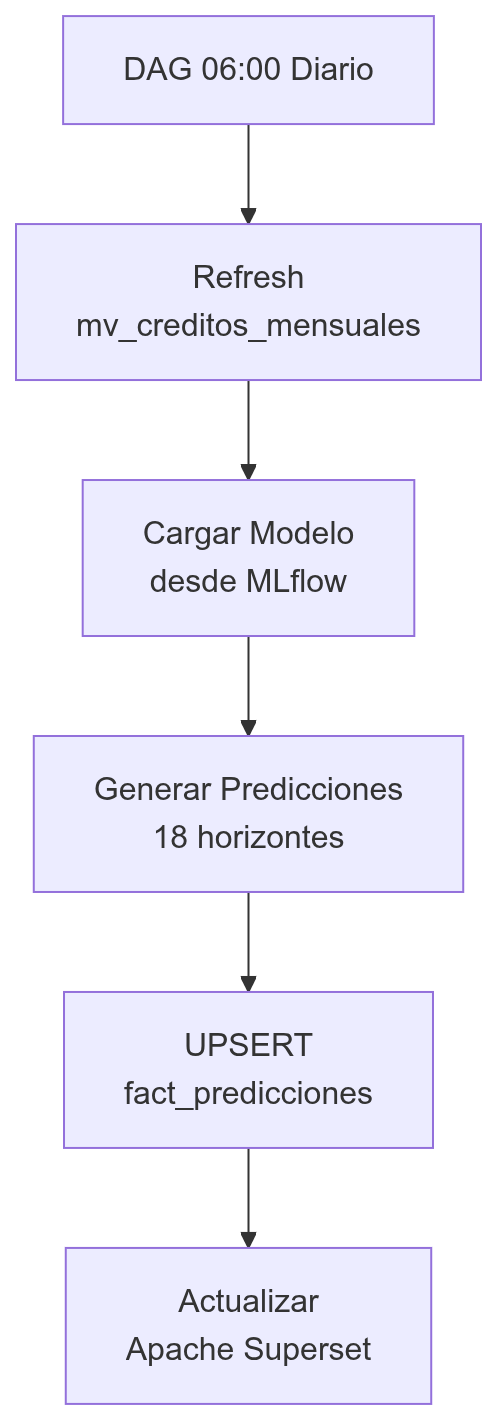
\includegraphics[width=0.8\linewidth]{images/MM-06 Flujo de Inferencia Diaria.png}
    \caption{Flujo de inferencia y actualización analítica. El DAG diario actualiza la vista materializada, carga el modelo y genera predicciones para los 18 horizontes.}
    \label{fig:inferencia}
\end{figure}

La tabla de predicciones contiene probabilidades \texttt{prob\_h01}--\texttt{prob\_h18}, predicciones binarias \texttt{pred\_h01}--\texttt{pred\_h18} con umbral 0,5, medidas resumen y metadatos de ejecución. El proyecto no presenta evaluación de calibración ni optimización del umbral, por lo que el valor 0,5 se considera una decisión de implementación y no un umbral de negocio validado.

\section{Diseño del datamart y dashboards}

El datamart adopta un esquema estrella con \texttt{dim\_tiempo}, \texttt{dim\_riesgo}, \texttt{dim\_sector} y \texttt{dim\_sucursal}. Las tablas \texttt{fact\_creditos\_mensual} y \texttt{fact\_predicciones\_mensual} almacenan los agregados históricos y las predicciones. Apache Superset consulta estas tablas para construir siete dashboards: histórico de créditos, análisis dimensional, KPIs generales, predicciones por sucursal, predicciones por sector, evolución temporal y bloques de mayor riesgo.

\begin{figure}[H]
    \centering
    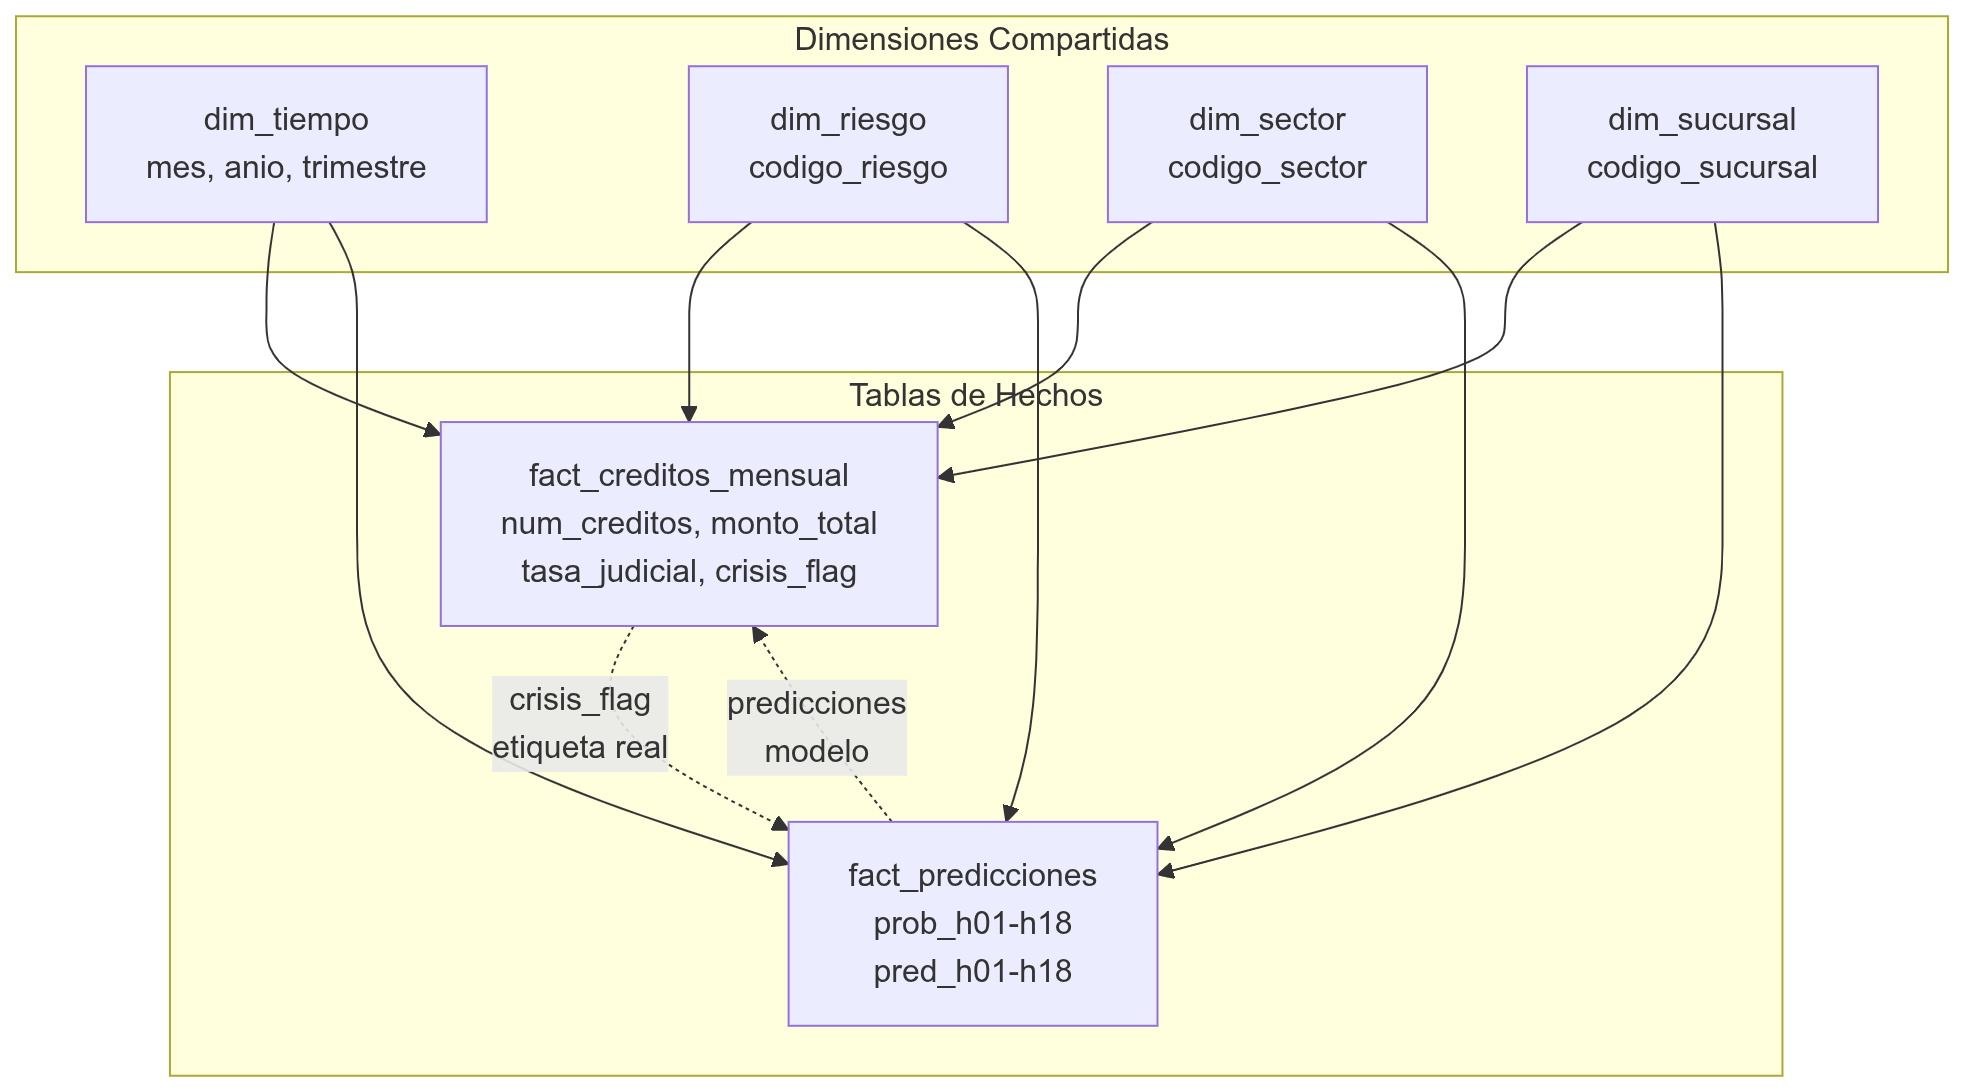
\includegraphics[width=0.6\linewidth]{images/MM-09 Diagrama de Integracion.png}
    \caption{Esquema conceptual del datamart analítico. Las dimensiones comparten ambas tablas de hechos: fact\_creditos\_mensual (datos históricos) y fact\_predicciones (salida del modelo).}
    \label{fig:datamart}
\end{figure}

\section{Recursos computacionales}

La Tabla 4.6 documenta los recursos utilizados para el entrenamiento de los modelos, extraída del código y la documentación del proyecto.

\begin{table}
\centering
\small
\begin{tabular}{|l|l|}
\hline
\textbf{Recurso} & \textbf{Especificación} \\
\hline
Procesador & [PENDIENTE: especificar CPU] \\
\hline
Memoria RAM & [PENDIENTE: especificar GB] \\
\hline
GPU & [PENDIENTE: especificar si aplica] \\
\hline
Sistema operativo & [PENDIENTE: especificar SO] \\
\hline
Python & 3.12 \\
\hline
TensorFlow/Keras & [PENDIENTE: versión] \\
\hline
LightGBM & [PENDIENTE: versión] \\
\hline
PostgreSQL & 15 \\
\hline
Apache Airflow & 2.10 \\
\hline
MLflow & [PENDIENTE: versión] \\
\hline
Apache Superset & [PENDIENTE: versión] \\
\hline
\end{tabular}
\caption{Recursos computacionales y versiones de software. Los campos marcados como [PENDIENTE] deben completarse con la información exacta del entorno de ejecución.}
\label{tab:recursos}
\end{table}

\textbf{Tiempos de ejecución reportados}: LightGBM entrenó los 18 horizontes en aproximadamente 5 minutos; CNN requirió más de 2 horas sin convergencia; MLP requirió un tiempo intermedio. Estos tiempos son aproximados y pueden variar según el hardware utilizado.

\section{Versionado y reproducibilidad}

El proyecto utiliza los siguientes mecanismos para garantizar la reproducibilidad:

\begin{itemize}
    \item \textbf{Semilla fija}: LightGBM utiliza \texttt{seed=42}; CNN y MLP no fijan semilla.
    \item \textbf{Registro en MLflow}: Cada ejecución registra parámetros, métricas y artefactos.
    \item \textbf{Contenedores Docker}: El proyecto incluye configuración para despliegue en contenedores.
    \item \textbf{Repositorio GitHub}: Código fuente disponible en el repositorio del proyecto.
\end{itemize}

\textbf{Limitaciones de reproducibilidad}: (1) CNN y MLP no fijan semilla, por lo que los resultados pueden variar entre ejecuciones; (2) no se documentan versiones exactas de todas las librerías; (3) no se adjunta el hardware específico utilizado; (4) no se preservan los datos originales por restricciones de confidencialidad.